\chapter{What a finite spectrum can tell us about a CFT}
\label{ch:scaling}

A finite quantum chain has a discrete spectrum whether its infinite-volume
limit is critical, massive, or separated from either regime by a long
crossover. The task is therefore not simply to find low energies. It is to
identify a scaling organization that persists as the circumference grows.
This chapter connects the cylinder formulas of CFT to measured lattice
quantities, derives several central-charge diagnostics, and explains the
different errors attached to an eigenpair, a variational state, and a
continuum extrapolation. The Haagerup chain provides useful examples because
its finite calculations can be very accurate while their limiting
interpretation remains unsettled.
The state-operator correspondence and cylinder transformation used
below were derived in Chapter~\ref{ch:cft}.

\section{The cylinder dictionary and its assumptions}
\index{finite-size scaling}

For a nonchiral CFT with $c_L=c_R=c$, the Hamiltonian on a circle of
circumference $L$ is
\begin{equation}
 H_{\mathrm{CFT}}=\frac{2\pi v}{L}
       \left(L_0+\bar L_0-\frac c{12}\right).
 \label{eq:cylinder-H-lattice}
\end{equation}
Here $v$ converts spatial and temporal units. A lattice Hamiltonian also
contains an extensive nonuniversal energy $e_\infty L$. Consequently a
critical periodic chain is expected to have
\begin{align}
 E_0(L)&=e_\infty L-\frac{\pi vc}{6L}+\cdots,\label{eq:casimir}\\
 E_a(L)-E_0(L)&=\frac{2\pi v}{L}
       \left(h_a+\bar h_a+n+\bar n\right)+\cdots.\label{eq:gap-dictionary}
\end{align}
The dots include corrections from irrelevant fields, running couplings,
microscopic geometry, and the approach to a possible fixed point. Their
form is extra information, not part of the leading formula.

An energy gap and a conformal scaling gap are different quantities.
A gapped chain has a positive lower bound on excitation energies above
its vacuum sector, independent of sufficiently large $L$ along a size
sequence compatible with the proposed order and boundary sector. With several
pure vacua, that sector may be a cluster of nearly degenerate
finite-volume states; their small internal splittings do not define
the bulk gap. A CFT may have a positive lowest nonidentity scalar
dimension $\Delta_{\min}$ while remaining gapless, since its
corresponding energy difference is $2\pi v\Delta_{\min}/L$.

Equation~\eqref{eq:gap-dictionary} assumes that one common velocity describes
the fields being compared. A system with decoupled sectors of different
velocities need not admit this single-cylinder interpretation before its
Hamiltonian is rescaled sector by sector. We also assume that the chosen
finite-volume state approaches the intended CFT vacuum.

The conformal dimension and spin are
\[
 \Delta=h+\bar h,\qquad s=h-\bar h.
\]
For descendants the changes are $\Delta\mapsto\Delta+n+\bar n$ and
$s\mapsto s+n-\bar n$. Near a microscopic carrier momentum $k_\star$, the
lattice momentum has the form
\begin{equation}
 k=k_\star+\frac{2\pi}{L}(s+n-\bar n)+\cdots.
 \label{eq:carrier-spin}
\end{equation}
The carrier matters in the Haagerup chain, whose low-energy states occur
near $0$ and the two commensurate momenta $\pm2\pi/3$. The momentum
relative to one of these cones is the quantity compared with conformal
spin. A state at total lattice momentum $2\pi/3$ can still be a residual
scalar.

For lengths not divisible by three, the carrier is incompatible with
periodic momentum quantization. Those lengths probe a different residual
translation boundary condition. They are valuable data, but their vacuum
energies and momentum offsets should not be pooled with the divisible
lengths without a twisted-sector dictionary.

\begin{example}[Ratios eliminate a common velocity]
If two tracked primary gaps obey the same leading formula, then
\[
 \frac{E_a-E_0}{E_b-E_0}\longrightarrow\frac{\Delta_a}{\Delta_b}.
\]
Neither the bulk energy nor $v$ occurs. If a separately identified stress
state has $\Delta_T=2$, one may define the finite diagnostic
\[
 \Delta_a^{(T)}(L)=2\frac{E_a(L)-E_0(L)}{E_T(L)-E_0(L)}.
\]
This removes an independently fitted velocity, but replaces it by the
assumption that the denominator tracks pure stress.
\end{example}

\section{Canonical calibration: the periodic critical Ising chain}
\label{sec:scaling-Ising}
\index{Ising model!critical chain}\index{Jordan--Wigner transformation}
\index{fermion parity}\index{Neveu--Schwarz sector}\index{Ramond sector}

Before analyzing an unfamiliar chain, it helps to run the cylinder
dictionary through a model whose finite spectrum can be found exactly.

\begin{example}[From a periodic spin spectrum to Ising CFT]
\label{ex:scaling-Ising-calibration}
Take Pauli matrices $\sigma_j^a$ and
\begin{equation}
 H_{\rm I}=-J\sum_{j=1}^L
       \left(\sigma_j^x\sigma_{j+1}^x+\sigma_j^z\right),
 \qquad J>0,\qquad \sigma_{L+1}^a=\sigma_1^a.
 \label{eq:scaling-Ising-H}
\end{equation}
The lattice spacing is one, so the circumference is $L$.
We take $L$ even; the displayed stress-pair construction below
uses $L\ge4$. The equality of the interaction and transverse-field
coefficients is the critical point in this Pauli-matrix convention.
Changing from Pauli matrices to spin operators $\sigma^a/2$ without
changing the couplings would change the normalization of every energy.

\paragraph{A periodic spin ring has two fermion boundary conditions.}

The conserved spin-flip parity is
$P=\prod_j\sigma_j^z$; here parity means internal spin flip,
not spatial reflection. Introduce Jordan--Wigner fermions
\[
 c_j=\left(\prod_{m<j}\sigma_m^z\right)\sigma_j^+,
 \qquad
 \sigma_j^+=\frac{\sigma_j^x+i\sigma_j^y}{2}.
\]
The string makes fermions on different sites anticommute.
At the same site,
\[
 n_j=c_j^\dagger c_j=\frac{1-\sigma_j^z}{2},
 \qquad P=(-1)^{\sum_jn_j}.
\]
For an interior bond the strings cancel to give
$\sigma_j^x\sigma_{j+1}^x
=(c_j^\dagger-c_j)(c_{j+1}^\dagger+c_{j+1})$.
Across the last bond their uncancelled product is the total
parity. The quadratic Hamiltonian therefore has the uniform form
\[
 H_{\rm I}=-J\sum_{j=1}^L
 \left[(c_j^\dagger-c_j)(c_{j+1}^\dagger+c_{j+1})
                  +1-2n_j\right],
 \qquad c_{L+1}=-P c_1,
\]
where the boundary sign is imposed within a fixed parity sector.
Consequently the physical Hilbert space is
\begin{equation}
 \HH_{\rm spin}
 =\HH_{\rm NS,\ even}\oplus\HH_{\rm R,\ odd}.
 \label{eq:scaling-Ising-parity}
\end{equation}
Here NS means antiperiodic fermions, the Neveu--Schwarz sector,
with momenta $k=(2n+1)\pi/L$. R means periodic fermions, the
Ramond sector, with $k=2n\pi/L$. These are two sectors of the
same periodic spin Hamiltonian. Each fermion Fock space must
still be projected to the indicated parity. Keeping both full
Fock spaces would count twice as many states as the $2^L$ spin
Hilbert space.

A Fourier transform leaves a two-mode problem for each pair
$k,-k$. In the basis $(c_k,c_{-k}^\dagger)$ its single-particle
matrix can be written
\[
 \mathsf h(k)=2J\left[(1-\cos k)\tau_z+\sin k\,\tau_y\right],
\]
where the $\tau$ matrices act on this particle-hole pair.
Its positive eigenvalue is
\begin{equation}
 \begin{aligned}
 \epsilon(k)&=2J\sqrt{(1-\cos k)^2+\sin^2k}\\
            &=4J\left|\sin\frac k2\right|.
 \end{aligned}
 \label{eq:scaling-Ising-dispersion}
\end{equation}
The associated Bogoliubov transformation mixes creation and
annihilation operators in opposite-momentum pairs and preserves
fermion parity. It is canonical: the new operators $\gamma_k$
obey the same fermion anticommutation relations. The diagonal form is
\[
 H_{\rm I}=\sum_k\epsilon(k)
              \bigl(\gamma_k^\dagger\gamma_k-\tfrac12\bigr),
\]
with each allowed quasiparticle momentum counted once. Its empty-mode
energy is therefore minus one half of the dispersion sum.
In the NS sector there are no unpaired $k=0,\pi$
modes for even $L$. Its Bogoliubov vacuum has even parity, and
each quasiparticle flips parity. Physical NS excitations must
therefore contain an even number of quasiparticles.

The Ramond sector requires more care. It contains unpaired
$k=0$ and $k=\pi$ modes, with terms
$2J(1-\cos k)(n_k-\tfrac12)$.
At criticality the $k=0$ term is exactly zero, whereas
$k=\pi$ costs $4J$ to occupy. The paired-mode vacuum has even
parity. The physical R ground state has the $\pi$ mode empty
and the zero mode occupied, supplying the required odd parity
at no energy cost. Thus its energy is the usual zero-point sum.
The two possible zero-mode occupations belong to different
fermion parities; they are not two physical R ground states
of the periodic spin problem.

\paragraph{Two finite trigonometric sums give the Casimir energy.}

Put $x=\pi/(2L)$. Choosing momenta in $[0,2\pi)$ makes every
sine in the zero-point sums nonnegative. The NS vacuum energy is
\[
 E_0(L)=-\frac12\sum_{k\in{\rm NS}}\epsilon(k)
        =-2J\sum_{n=0}^{L-1}\sin[(2n+1)x].
\]
The elementary identity
$2\sin x\sin y=\cos(y-x)-\cos(y+x)$ telescopes:
\[
 2\sin x\sum_{n=0}^{L-1}\sin[(2n+1)x]
 =\cos0-\cos(2Lx)=2.
\]
Therefore
\begin{equation}
 E_0(L)=-2J\csc\frac{\pi}{2L}.
 \label{eq:scaling-Ising-E0}
\end{equation}
The same argument in the physical R sector gives
\[
 2\sin x\sum_{n=0}^{L-1}\sin(2nx)
 =\cos(-x)-\cos[(2L-1)x]=2\cos x,
\]
and hence
\begin{equation}
 E_{\rm R}(L)=-2J\cot\frac{\pi}{2L}.
 \label{eq:scaling-Ising-ER}
\end{equation}
The zero-mode occupation changes no term in this sum.
Since $\csc x>\cot x$ for the present $x$, the NS state is the
ground state of the full spin Hamiltonian.

The small-momentum slope of the exact dispersion gives an
independent velocity:
\[
 \epsilon(k)=2J|k|-\frac J{12}|k|^3+O(|k|^5),
 \qquad v=2J.
\]
Using $\csc x=x^{-1}+x/6+7x^3/360+O(x^5)$,
\begin{equation}
 E_0(L)=-\frac{4J}{\pi}L-\frac{\pi J}{6L}
        -\frac{7\pi^3J}{1440L^3}+O(L^{-5}).
 \label{eq:scaling-Ising-Casimir}
\end{equation}
Thus $e_\infty=-4J/\pi$. Comparing the $L^{-1}$ coefficient
with $-\pi vc/(6L)$, using the independently known $v=2J$,
gives $c=1/2$. The coefficient alone would only have given
$vc=J$. The long-wavelength modes form a massless Majorana
fermion, providing an independent continuum description with
the same central charge.

Even here a finite-size central-charge estimator is not exactly
its limiting value. If the exact $e_\infty$ and $v$ are used,
\[
 -\frac{6L}{\pi v}\bigl[E_0(L)-e_\infty L\bigr]
 =\frac12+\frac{7\pi^2}{480L^2}+O(L^{-4}).
\]
The correction is a property of an exactly solved finite
Hamiltonian, not an eigensolver error.

\paragraph{The spin, energy, and stress levels.}

The odd-parity ground lies above the NS ground by
\begin{equation}
 g_\sigma(L):=E_{\rm R}(L)-E_0(L)
 =2J\bigl(\csc x-\cot x\bigr)
 =2J\tan\frac x2.
 \label{eq:scaling-Ising-spin-gap}
\end{equation}
The last equality uses
$(1-\cos x)/\sin x=\tan(x/2)$.
In particular,
\[
 g_\sigma(L)=\frac{\pi J}{2L}
             +\frac{\pi^3J}{96L^3}+O(L^{-5}),
 \qquad
 \frac{L g_\sigma(L)}{2\pi v}
 =\frac18+\frac{\pi^2}{384L^2}+O(L^{-4}).
\]
This is the Ising spin-field sector, with limiting
$(h,\bar h)=(1/16,1/16)$. The sector identification has more
content than an energy fit: the lattice order operator
$\sigma_j^x$ changes $P$, and its Jordan--Wigner string changes
the Majorana boundary condition between NS and R.
In the continuum this boundary-condition change is the spin
field. Both parity-sector ground states have physical momentum
zero. One can see this directly in the spin basis: the
off-diagonal matrix elements are nonpositive, adjacent pair
flips connect each fixed-parity sector, and its positive ground
vector is invariant under translation.

In the NS sector a single quasiparticle at $k=\pi/L$ is
not a physical periodic-spin state: it has the wrong parity.
The allowed opposite-momentum pair at $k=\pm\pi/L$ has
zero total momentum and gap
\begin{equation}
 g_\epsilon(L)=2\epsilon(\pi/L)=8J\sin x.
 \label{eq:scaling-Ising-energy-gap}
\end{equation}
Its known-velocity dimension estimate is
\begin{equation}
 \Delta_\epsilon^{(v)}(L)
 :=\frac{L g_\epsilon(L)}{2\pi v}
 =\frac{2L}{\pi}\sin\frac{\pi}{2L}
 =1-\frac{\pi^2}{24L^2}+O(L^{-4}).
 \label{eq:scaling-Ising-epsilon-v}
\end{equation}
In the Majorana continuum theory this pair is
$\psi_{-1/2}\bar\psi_{-1/2}|0\rangle$, with weights
$(1/2,1/2)$: the energy field $\epsilon$.

The same-direction pair at $k=\pi/L,3\pi/L$ is also allowed.
Its total momentum is $4\pi/L$ modulo $2\pi$, and its gap is
\begin{align}
 g_T(L)&=4J(\sin x+\sin3x)
        =16J\sin x\cos^2x,\label{eq:scaling-Ising-stress-gap}\\
 \frac{Lg_T(L)}{2\pi v}
       &=2-\frac{7\pi^2}{12L^2}+O(L^{-4}).\notag
\end{align}
The momenta correspond to continuum half-integer fermion modes
$1/2$ and $3/2$. This identifies the limiting state, rather
than merely matching its momentum. With
$\{\psi_r,\psi_s\}=\delta_{r+s,0}$ and
$T=-\tfrac12:\!\psi\partial\psi\!:$,
\[
 L_{-2}|0\rangle
 =\frac12\psi_{-3/2}\psi_{-1/2}|0\rangle.
\]
The two-fermion vector has norm one, so the stress state has
norm squared $1/4=c/2$, as required by the Virasoro algebra.
Its weights are $(2,0)$ and its spin is $+2$.
The negative-momentum pair gives the opposite chirality.
At $L=4$ the total lattice momenta of the two opposite-chirality
pairs coincide modulo $2\pi$;
their distinct continuum chiral labels should not be inferred
from that short-ring momentum alone.

The parity projection also explains the bosonic local
continuum spectrum. Even-even chiral NS fermion parity gives
the vacuum family, and odd-odd chiral NS parity gives the
energy family. The projected R space gives the spin family.
Thus its continuum Hilbert space is
\[
 \HH_{\rm Ising}
 =\bigl(\mathcal V_0\otimes\overline{\mathcal V_0}\bigr)
  \oplus\bigl(\mathcal V_{1/2}
                   \otimes\overline{\mathcal V_{1/2}}\bigr)
  \oplus\bigl(\mathcal V_{1/16}
                   \otimes\overline{\mathcal V_{1/16}}\bigr),
\]
where $\mathcal V_h$ is the irreducible Ising Virasoro module.
An unprojected single chiral fermion of spin $1/2$ is not an
additional local field in this periodic bosonic theory.

\paragraph{Two legitimate calibrations approach from opposite sides.}
\index{velocity!finite-size calibration}

The exact velocity $v=2J$ is an infinite-volume slope. A
stress-gap estimate uses a different quantity,
\[
 \widehat v_T(L):=\frac{Lg_T(L)}{4\pi}
 =\frac{4JL}{\pi}\sin x\cos^2x
 =2J\left[1-\frac{7\pi^2}{24L^2}+O(L^{-4})\right].
\]
It tends to $v$, but differs from it at every finite size.
Using this estimate to normalize the energy-field gap gives
\begin{equation}
 \Delta_\epsilon^{(T)}(L)
 :=\frac{L g_\epsilon(L)}{2\pi\widehat v_T(L)}
 =2\frac{g_\epsilon(L)}{g_T(L)}
 =\sec^2\frac{\pi}{2L}
 =1+\frac{\pi^2}{4L^2}+O(L^{-4}).
 \label{eq:scaling-Ising-epsilon-stress}
\end{equation}
The exact identity follows by cancelling $\sin x$ between
$g_\epsilon=8J\sin x$ and $g_T=16J\sin x\cos^2x$.
The known-velocity estimate
\eqref{eq:scaling-Ising-epsilon-v} approaches dimension one
from below; the stress-calibrated estimate approaches it from
above. They use the same exact eigenvalues and track the same
limiting field. Removing the velocity by a ratio does not
remove the unequal finite-size corrections of the two levels.

For this nearest-neighbor Ising Hamiltonian the corrections can
be derived from the full dispersion and the finite sums:
the cubic term in $\epsilon(k)$ produces $L^{-3}$ corrections
to gaps and hence $L^{-2}$ corrections to dimension estimates.
That power is consistent with dimension-four irrelevant
contributions in a continuum expansion, but the power alone
does not specify a unique irrelevant operator.
Other Hamiltonians can have different coefficients, vanishing
leading coefficients, or logarithmic running such as the
current example in Chapter~\ref{ch:full_theories}.

This calibration illustrates what becomes possible when the
boundary conditions, parity projection, velocity, eigenstates,
and continuum field dictionary are all independently controlled.
For the Haagerup chain, exact finite eigenvalues or a small
residual do not supply those missing identifications. Its
finite-size analysis must still determine which sectors
approach a common vacuum and velocity, which states approach
the proposed fields, and what correction law governs that
approach.
\end{example}

\begin{figure}[tbp]
 \centering
 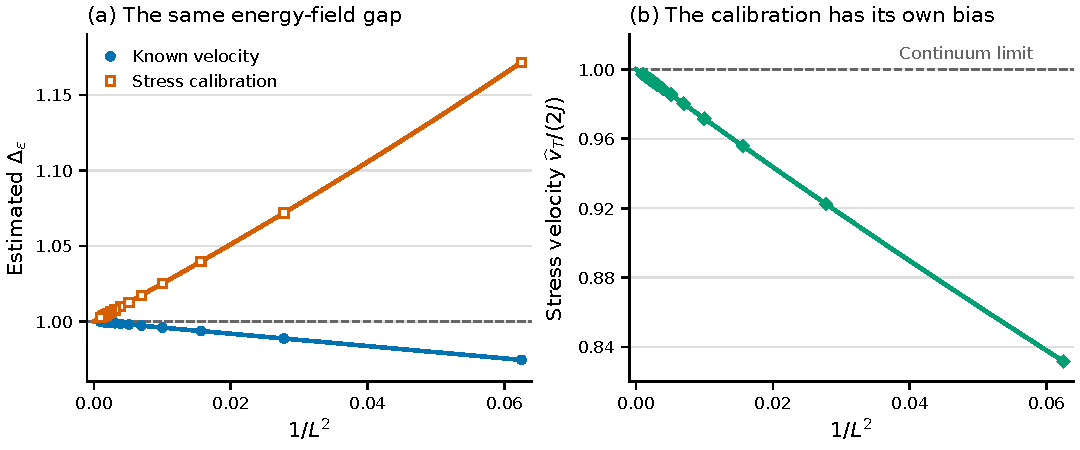
\includegraphics[width=\textwidth]{figures/ising_calibration.pdf}
 \caption{Two finite-size calibrations of the same critical Ising
 energy-field gap, using the exact formulas in
 Example~\ref{ex:scaling-Ising-calibration}.
 Symbols mark even $L=4,6,\ldots,32$; curves show the smooth
 continuation of the formulas to real $L\geq4$.
 Put $z=\pi/(2L)$. The known-velocity estimate is
 $\Delta_\epsilon^{(v)}=\sin z/z$, whereas the stress-calibrated
 estimate is $\Delta_\epsilon^{(T)}=\sec^2z$.
 They approach the same dimension from opposite sides.
 The right panel shows the calibration bias itself:
 $\widehat v_T/(2J)=(\sin z/z)\cos^2z$.
 Dashed lines show the common limiting value~$1$ at $1/L^2=0$.
 These are exact Ising formulas, not fits or Haagerup-chain data.}
 \label{fig:scaling-Ising-calibrations}
\end{figure}

\section{An accurate eigenpair is a finite statement}

Suppose a normalized numerical vector $u$ has Rayleigh value $E$ and
residual $r=(H-E)u$. In a finite Hermitian problem,
\begin{equation}
 \operatorname{dist}(E,\operatorname{spec}H)\leq\|r\|.
 \label{eq:residual-spectrum}
\end{equation}
To prove this, expand $u=\sum_nc_n|n\rangle$ in an exact eigenbasis. Then
$\|r\|^2=\sum_n|c_n|^2(E_n-E)^2$. If every exact energy were farther
than $\|r\|$, the weighted average would be larger than $\|r\|^2$.

This useful bound does not establish that the nearby eigenvalue is the
lowest one in a sector, that all lower levels have been found, or that the
state has a particular conformal identity. With an independent spectral
gap separating a target eigenspace from the rest, one can turn a residual
into a bound on the unwanted component of $u$. Without such separation,
nearly degenerate eigenvectors can rotate substantially while their
energies remain accurate.

For a variational normalized state $u$, the energy is an upper bound on the
ground energy in the allowed Hilbert space. A difference of two variational
energies is generally not an upper or lower bound on an excitation gap:
the two approximation errors can have either ordering. A small optimizer
gradient tests stationarity within the chosen coordinates, and a small
variance tests closeness to some energy eigenspace. Neither alone proves
global minimality.

\begin{remark}[Three separate questions]
A useful report answers three questions separately: how accurately was a
finite matrix problem solved; how completely were its relevant sectors
covered; and how well is the infinite-size correction law controlled?
Many significant mistakes arise by answering the third question with an
impressive number from the first.
\end{remark}

\section{Casimir energy: why the velocity remains}
\index{Casimir energy}

Divide \eqref{eq:casimir} by $L$ and write $x=L^{-2}$. The leading relation
is a line,
\[
 \frac{E_0(L)}L=e_\infty-\frac{\pi vc}{6}x+\cdots.
\]
Its slope determines the product $vc$. The ground-state energy alone does
not distinguish a larger central charge with a smaller velocity from a
smaller central charge with a larger velocity.

The stored small-chain ground energies for the physical $\mathcal H_3$ model are
\[
 E_0(3)=-3,\quad E_0(6)=-5.271980047610,\quad
 E_0(9)=-7.737524752482.
\]
The reported length-three value saturates the local lower bound at
the displayed precision. A two-size fit using $6,9$ gives the descriptive value
$vc=2.34379137903$. With two observations and two unknown coefficients
the line interpolates exactly. An exact interpolation is not evidence
that the omitted terms vanish.

One way to estimate $v$ is to identify a conformal level with known
dimension. Another is to compare independently normalized energy and
current responses. Both approaches need a field dictionary. Inferring
$v$ by declaring the first convenient momentum-two state to be stress
builds the desired answer into the normalization.

\section{Deriving the stress-source estimator}
\index{stress-source estimator}

Use the energy Fourier mode $H_2$ of \eqref{eq:energy-Fourier}. Under a
specific lattice-to-CFT identification of the energy density,
\begin{equation}
 H_2\longrightarrow\frac{2\pi v}{L}(L_{-2}+\bar L_2).
 \label{eq:stress-mode-assumption}
\end{equation}
Acting on the vacuum, the second term vanishes. The Virasoro commutator
\[
 [L_2,L_{-2}]=4L_0+\frac c2
\]
therefore gives $\|L_{-2}|0\rangle\|^2=c/2$. For a unit-normalized
stress state $|T\rangle$, put
$M=\langle T|H_2|0\rangle$ and $g_T=E_T-E_0$. The ideal cylinder
formulas are
\[
 |M|^2=\left(\frac{2\pi v}{L}\right)^2\frac c2,
 \qquad g_T=\frac{4\pi v}{L}.
\]
Dividing cancels the unknown velocity:
\begin{equation}
 \widehat c_T(L)=\frac{8|M|^2}{g_T^2}.
 \label{eq:stress-c-estimator}
\end{equation}
There is no extra factor of two for the opposite chirality. A complex
Fourier mode of the stated sign creates one chiral stress state from the
vacuum under this identification. On a ring so short that the two
Fourier labels coincide, such as $m=2$ and $m=-2$ at $L=4$, the
source momentum alone cannot establish its chirality.

\begin{numericalrecord}[Measured stress candidates]
The physical-chain calculation uses the neutral momentum-two sector and
selects a low-energy state with large overlap with $H_2|0\rangle$. The
following are saved finite results, not extrapolated central charges:
\begin{center}
\begin{tabular}{c r r r}
$L$ & $g_T$ & $|M|^2$ & $\widehat c_T(L)$\\\hline
6 &1.271980047610&1.159949183395&5.735461284\\
9 &1.153308959914& .516954434465&3.109216187\\
12& .950908727688& .293569361127&2.597305575\\
15& .793841246905& .189323099189&2.403401186
\end{tabular}
\end{center}
The later $L=18$ continuation has $g_T=.6768446828683299$ and conditional
$\widehat c_T(18)\simeq2.30768$, with a full eigenpair residual of order
$4\times10^{-14}$. Its stress-source fraction is approximately $.95444$.
\end{numericalrecord}

The dominant state in the older calculations is not the lowest state at
momentum two. This alone is an important lesson: lattice momentum does
not identify a conformal family. If several states form a nearly
degenerate candidate stress cluster, the basis-independent overlap is
the sum of their squared amplitudes. But this sum equals stress weight
only if other contributions to the cluster have been excluded or
separated.

\subsection{Energy-density improvements}

The periodic sum is unchanged under
\[
 h_j\mapsto h_j+B_{j+1}-B_j.
\]
For the Fourier mode with $k=2\pi m/L$, the change is
\[
 \delta H_m=(e^{ik}-1)\sum_j e^{-ikj}B_j.
\]
If $B$ has a continuum field of dimension $\Delta_B$, its extensive
Fourier mode scales as $L^{1-\Delta_B}$, and the finite difference
contributes another $L^{-1}$. Thus $\Delta_B=1$ gives the same $L^{-1}$
scaling as the stress mode. A current descendant can contaminate a
dimension-two source without changing the total Hamiltonian.

For a correctly separated pure stress eigenstate, an orthogonal current
descendant does not change the stress matrix element. The difficulty is
establishing that separation. Largest-overlap selection and high captured
source weight are evidence about a finite source, not a proof of
\eqref{eq:stress-mode-assumption}.

\subsection{If the limiting ground is not the identity}
\index{effective central charge}

The vacuum hypothesis is substantive. Suppose instead that the
regulated ground states approach a spin-zero highest-weight
threshold with $h=\bar h=h_0>0$. Its cylinder energy would involve
\[
 c_{\mathrm{eff}}=c-24h_0
\]
in the Casimir term. The Virasoro algebra, however, still has
central charge $c$. Its descendants obey
\[
 \|L_{-1}|h_0\rangle\|^2=2h_0,\qquad
 \|L_{-2}|h_0\rangle\|^2=4h_0+c/2.
\]
Thus the ground must have a nonzero same-symmetry momentum-one
descendant at relative dimension one, provided the regulated
low-energy stress action converges. A controlled sum of its
level-two stress-source weight would return $c+8h_0$ under the
vacuum estimator normalization, not $c_{\mathrm{eff}}$.

The sum matters: above a nonvacuum primary, the level-two space
contains both $L_{-2}|h_0\rangle$ and $L_{-1}^2|h_0\rangle$,
which are not orthogonal in general. Their Gram matrix is the one
derived in Chapter~\ref{ch:cft}. One selected lattice eigenstate
need not carry all the $L_{-2}$ weight.

For a concrete proposed mechanism, the bosonic cigar has
\[
 c=2+\frac6{k-2},\qquad h_0=\frac1{4(k-2)},\qquad
 c_{\mathrm{eff}}=2.
\]
Its identity is not normalizable; regulated radial levels approach
a continuum threshold. Hence a Casimir estimate near two is
compatible with a larger Virasoro charge in that theory. It also
brings extra obligations: level-one spectral weight and a growing
density of radial states. Under the simplest angular-charge
assignment, a charged scalar of threshold-relative dimension
$1/(2k)$ equal to $1/8$ would fix $k=4$, giving
$c=5$, $h_0=1/8$, and $c+8h_0=6$.

At $L=9,12,15$, the saved first fully Haagerup-invariant momentum-one
gaps have effective dimensions about $2.800,2.846,2.884$, using
the saved epsilon-descendant velocity calibration. They do not
display the required threshold descendant near dimension one in
the observed regime. This is a conditional diagnostic,
since logarithmic convergence can be slow and the low-energy
stress map itself needs control. It does not exclude every
noncompact CFT or license replacing $c$ by $c_{\mathrm{eff}}$ in
the vacuum sewing formulas.

The named calibration assumes that a selected momentum-one level is
the first descendant of the neutral scalar $\epsilon$: its gap from
that scalar is set equal to $2\pi v/L$. This is a different finite-size
prescription from setting the stress gap equal to $4\pi v/L$.

\section{Entropy on a finite ring}

For an interval of length $\ell$ in a periodic ground state, the CFT
formula is
\begin{equation}
 S_L(\ell)=\frac c3\log\left[\frac L\pi
       \sin\left(\frac{\pi\ell}L\right)\right]+s_0+\cdots.
 \label{eq:periodic-entropy}
\end{equation}
The logarithm contains the chord length, not simply $\ell$. At small
$\ell/L$ it approaches $\log\ell$; near the midpoint it reflects the
finite circumference. An additive entropy constant can be eliminated by
comparing two cuts or two sizes, but cutoff and boundary corrections
remain.

For the stored ordinary height-embedding entropies,
\[
 S_6(3)=2.258824289079,\qquad S_9(4)=2.529902677312.
\]
Since the nine-site ring has no integer cut at exactly $L/2$, the
appropriate denominator in the two-size slope uses the actual chord
lengths. This gives the effective value $c=2.08438313923$. Replacing
$\sin(4\pi/9)$ by one introduces a small but avoidable geometric error.

This attractive number is not by itself a central-charge determination.
Within each size, fits over cuts $\ell\geq2$ give approximately $3.3880$
at $L=6$ and $2.7302$ at $L=9$; the first fit has only two points.
Different cut residues, short distances, and finite-size corrections
clearly matter. A visually smooth curve and a close rational or integer
slope do not bound them.

The partial trace convention must also be specified. The displayed
entropies arise from the ordinary embedding in $(\C^6)^{\otimes L}$.
An anyonic partial trace can add quantum-dimension boundary weights.
These constructions may share a leading universal logarithm under
appropriate hypotheses, but their finite entropies need not agree. One
must not combine their constants or finite slopes as though they were
the same observable.
Chapter~\ref{ch:tensor_networks} explains the ordinary Schmidt spectrum
and the extra entropy of a symmetry cat.

\subsection{An open-chain caution}

For an open critical chain the leading coefficient is $c/6$, rather
than $c/3$. Boundary degrees of freedom also contribute entropy. In an
open $\mathcal H_2$ representation related to a real-$q$ spin-one chain, a low
$S^z=0$ state showed substantial entropy growth from length $48$ to
$96$, while its low $S^z=1$ partner changed its midpoint entropy by
only about $.00764$. The nearly polarized edge state removes most of
the apparent growth. This is evidence about boundary-sensitive
finite-chain states in the $\mathcal H_2$ model, not a conclusion about $\mathcal H_3$.
Its pedagogical point is general: a boundary cat or entangled edge pair
can imitate bulk critical entropy over a long range.

\section{A thermal modular test using the whole spectrum}
\index{thermal modular moments}

Modular invariance supplies a different consistency test. Let
$g_a=E_a-E_0$ run through every state in the untwisted periodic
Hilbert space, with all charge and momentum multiplicities. At
inverse temperature $\beta$, define
\[
 Z_{\mathrm{gap}}(\beta)=\sum_a e^{-\beta g_a}.
\]
In a compact CFT with the vacuum identified and one velocity,
restoring the cylinder vacuum energy gives
\[
 Z(\beta)=e^{\beta a}Z_{\mathrm{gap}}(\beta),\qquad
 a=\frac{\pi cv}{6L}.
\]
The exchange of the two torus cycles maps
$\beta\mapsto L^2/(v^2\beta)$. At its fixed point
$\beta_*=L/v$, the function $Z(\beta_*e^t)$ is even in $t$. Its odd
derivatives therefore vanish.
This physical inverse temperature corresponds to the dimensionless
$b=2\pi$ of Chapter~\ref{ch:full_theories}.
The exchange is the same torus $S$ operation introduced in
Chapter~\ref{ch:cft}; projecting onto one ordinary charge sector
would generally transform to a different, spatially twisted trace.

Let $\mu=\langle g\rangle_{\beta_*}$ and
$m_j=\langle(g-\mu)^j\rangle_{\beta_*}$ in the probability distribution
proportional to $e^{-\beta_*g}$. The first derivative gives $a=\mu$,
or
\begin{equation}
 c=\frac{6\beta_*\mu}{\pi}.
 \label{eq:thermal-modular-c}
\end{equation}
The third derivative uses
$(\beta\partial_\beta)^3=
\beta\partial_\beta+3\beta^2\partial_\beta^2+
\beta^3\partial_\beta^3$.
After imposing $a=\mu$, it becomes
\begin{equation}
 \beta_*m_3=3m_2.
 \label{eq:thermal-modular-third}
\end{equation}
One can use this condition to seek $\beta_*$ without first choosing a
particular stress state. But the fifth derivative is an independent
requirement:
\[
 15\beta_*^2m_2-25\beta_*^3m_3+10\beta_*^4m_4-\beta_*^5m_5=0.
\]
Solving the third condition does not enforce the fifth.

For the physical chain, the root near velocity one gives effective
charges
\[
 c_6=2.31250,\qquad c_9=2.24215,\qquad c_{12}=2.19799
\]
in the stored diagnostic. Length six uses the complete spectrum; the
larger rings use specified low-state cutoffs in every ordinary
sector. The fifth condition remains unsatisfied. A compact-boson
control reproduces $c=1$ and its higher conditions, so the
construction of the diagnostic itself has a useful independent
check.

High moments amplify spectral tails. A tiny omitted contribution
to $Z_{\mathrm{gap}}$ can have a much larger effect on $m_5$.
Tail bounds require both a bound on how many states remain and a
genuine lower bound on their energies. Small residuals of the
retained eigenvectors supply neither completeness nor that lower
threshold. These modular equations are continuum requirements
tested on finite spectra; they are not exact identities of a
generic finite lattice Hamiltonian.

\section{Why fitting more decimals does not control the limit}

For the stress values above, choose the illustrative variable $x=L^{-2}$.
A linear fit through sizes $9,12,15$ gives intercept $1.989673$; a line
through $12,15$ gives $2.058682$; a quadratic through $9,12,15$ gives
$2.125928$. Two of these prescriptions interpolate their data exactly,
with no remaining fit degrees of freedom.

\begin{proposition}[Finite interpolation does not determine a limit]
Let $f(x_i)=y_i$ be prescribed at finitely many distinct positive points
$x_i$. If $p$ interpolates those data, then
\[
 p_\lambda(x)=p(x)+\lambda\prod_i(x-x_i)
\]
has exactly the same data for every $\lambda$, while $p_\lambda(0)$ can
take any value.
\end{proposition}
\begin{proof}
The added product vanishes at each observed point and is nonzero at
zero. Varying its coefficient changes the unobserved intercept freely.
\end{proof}

The proposition does not say all extrapolation is useless. A known
correction exponent, a controlled remainder, monotonicity, or a
renormalization-group analysis can rule out much of this freedom.
It says those are the ingredients that justify an extrapolation. Small
eigensolver residuals cannot substitute for them. Marginally irrelevant
operators can produce logarithmic corrections that look nearly
polynomial over accessible sizes, while a large finite correlation
length can produce a broad apparently critical window.

An honest comparison therefore retains several prescribed scales and
fit windows, rather than choosing the one nearest a desired value.
The spread is a sensitivity diagnostic. Without a justified model for
the corrections it is not a statistical confidence interval.

\section{Tracking light fields across sectors}

The Greek letters in this inventory label tracked Haagerup-chain
states. In particular, $\epsilon$ does not identify a state with the
Ising energy field of Example~\ref{ex:scaling-Ising-calibration}.

The completed ordinary-sector inventory at lengths $9,12,15$ covers
all $27,36,45$ intrinsic-charge and momentum sectors. It finds finite
light-shell multiplicities $2$ for $\phi$, $2$ for $\chi$, $4$ for
$\psi,\eta$ and their adjoints, and $1$ for $\epsilon$. The neutral
cone pair $\chi,\chi^\dagger$ must not be confused with the higher
invariant scalar accessed by a unit-channel source.
Here $\phi$ labels the lowest intrinsic-charge pair, $\chi$ the
intrinsically neutral pair at the nonzero carriers, and $\epsilon$
the low neutral scalar. Their full charge pattern and normalized
matrix elements are introduced in Chapter~\ref{ch:overlaps}.

\begin{numericalrecord}[Velocity-independent gap ratios]
The saved ratios are
\begin{center}
\begin{tabular}{c c c c}
 & $L=12$ & $L=15$ & $L=18$\\\hline
$g_\chi/g_\phi$&1.77474751&1.78423508&1.79085991\\
$g_\epsilon/g_\phi$&1.96087659&1.96657684&1.97006943\\
$g_\chi/g_\epsilon$&.90507863&.90727962&.90903391
\end{tabular}
\end{center}
At $L=18$, $g_\phi=.048135824413041206$,
$g_\chi=.08620451829960096$, and
$g_\epsilon=.0948309161570915$.
\end{numericalrecord}

These data make the fields' relative separation concrete without a
velocity assumption. They also show continuing drift. Finite shell
multiplicities are not a theorem about the complete continuum scalar
spaces. An unseen level can descend, an accidental degeneracy can
develop, and finite scalar assignments can mix with descendants.
Nevertheless, a complete finite-sector census is stronger evidence
than following only a favored charge line.

The source-visible invariant singlet gives another useful example. Its
stress-normalized dimension decreases from $2.29254$ to $2.22221$ to
$2.18339$ at $L=12,15,18$. Several formal $L^{-2}$ intercepts lie near
$2.095$, while independent amplitude-based effective dimensions lie
near $2.030$, $2.053$, and $2.082$. This is a field near the marginal
threshold in finite diagnostics. It does not establish an exactly
marginal scalar, a limiting dimension above two, or a beta function.

\section{Exercises}

\begin{exercise}\label{ex:scaling-residual}
Prove \eqref{eq:residual-spectrum}. Suppose in addition that every
eigenvalue outside a specified target cluster is at least $\gamma$
from $E$. Bound the squared norm of the component of $u$ outside that
cluster in terms of $\|r\|$ and $\gamma$.

\par\smallskip\noindent{\footnotesize\normalfont
\hyperref[sol:ex:scaling-residual]{Solution on page~\pageref*{sol:ex:scaling-residual}.}}\par
\end{exercise}
\begin{exercise}\label{ex:scaling-stress}
Derive \eqref{eq:stress-c-estimator} directly from the Virasoro
commutator. Repeat the calculation for a vacuum mode $L_{-n}$ and
derive its squared norm $c n(n^2-1)/12$.

\par\smallskip\noindent{\footnotesize\normalfont
\hyperref[sol:ex:scaling-stress]{Solution on page~\pageref*{sol:ex:scaling-stress}.}}\par
\end{exercise}
\begin{exercise}\label{ex:scaling-improvement}
Verify the Fourier transformation of $B_{j+1}-B_j$. For a continuum
field of dimension $\Delta_B$, explain the scaling of its contribution
to $H_m$ when $m$ is fixed as $L\to\infty$.

\par\smallskip\noindent{\footnotesize\normalfont
\hyperref[sol:ex:scaling-improvement]{Solution on page~\pageref*{sol:ex:scaling-improvement}.}}\par
\end{exercise}
\begin{exercise}\label{ex:scaling-casimir}
Use two sizes $L_1,L_2$ to eliminate $e_\infty$ in
\eqref{eq:casimir}. Write the resulting expression for $vc$ and
identify the combination of omitted corrections that survives.

\par\smallskip\noindent{\footnotesize\normalfont
\hyperref[sol:ex:scaling-casimir]{Solution on page~\pageref*{sol:ex:scaling-casimir}.}}\par
\end{exercise}
\begin{exercise}\label{ex:scaling-fraction}
An observed state has momentum one and gap corresponding to
$\Delta_\phi+1$ in a chosen scale. Compare its putative weights as
$L_{-1}\phi$ with those of a chiral current. Why does proximity to
that gap fail to establish a current?

\par\smallskip\noindent{\footnotesize\normalfont
\hyperref[sol:ex:scaling-fraction]{Solution on page~\pageref*{sol:ex:scaling-fraction}.}}\par
\end{exercise}
\begin{exercise}\label{ex:scaling-modular}
Derive the first, third, and fifth thermal modular conditions from
the evenness of $Z(\beta_*e^t)$. Explain why a partition function restricted
to the intrinsic neutral sector alone need not satisfy them.

\par\smallskip\noindent{\footnotesize\normalfont
\hyperref[sol:ex:scaling-modular]{Solution on page~\pageref*{sol:ex:scaling-modular}.}}\par
\end{exercise}
